\documentclass{beamer}
\mode<presentation>
\usetheme{CambridgeUS}
\usecolortheme{beaver}
\setbeamertemplate{caption}[numbered]

\usepackage[english]{babel}
\usepackage{graphicx}
\usepackage{subfigure}
\usepackage{url}
\usepackage[backend=bibtex, style=verbose]{biblatex}
\usepackage{multicol}
\bibliography{bibliography.bib}
\usepackage[noend]{algorithm,algpseudocode}


\title[LSTM: A Search Space Odysseys]{LSTM: A Search Space Odysseys}
\author[Mu\c sat Bogdan-Adrian]{Mu\c sat Bogdan-Adrian}
\date{February 2017}

\beamertemplatenavigationsymbolsempty
\graphicspath{{./images/}}

\begin{document}

\frame{\titlepage}

\begin{frame}
\frametitle{Recurrent Neural Networks - RNNs}
\center
\begin{itemize}
	\item Used to deal with sequential data, where there is a temporal dependence from a time instance to another
	\item Mathematically, they model a conditional distribution of the form \(P(x_t \lvert x_{t-1},..., x_2, x_1) \), where \(x_t\) is the current input at time \(t\)
	\item The output of a vanilla RNN cell at each time step is computed using the current input \(x_t\) and also the previous cell state \(h_{t-1}\)\footnote{Meant to encompass a summary of the past information} as:
	\[
		y_t = tanh(Ux_t + Wh_{t-1} + b),
	\]
	where \(U \in R^{M \times N}\), \(W \in R^{N \times N}\) are the shared parameter matrices for the RNN cells and \(b \in R^N\) is the bias
\end{itemize}
\end{frame}

\begin{frame}
\frametitle{Recurrent Neural Networks Unrolled}
\begin{figure}
	\subcapcentertrue
    \centering
    	\subfigure[RNN unrolled \footcite{Goodfellow-et-al-2016}] 
        {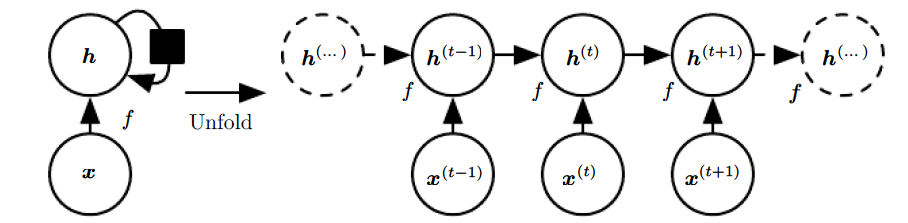
\includegraphics[width=0.7\textwidth]{rnn_unrolled.png}}
    \end{figure}
\end{frame}

\begin{frame}
\frametitle{Vanishing/Exploding Gradient}
\begin{itemize}
	\item The main algorithm for learning the weights of an RNN is called Backpropagation Through Time (BPTT)
	\item When computing the gradients with respect to the weights of the network, \(W\) depends on a recurrent connection from a previous timestep and so the partial derivative w.r.t. \(W\) becomes:
	\[
		\frac{\partial L^{(t)}}{\partial W} = \sum_{k=0}^{t} \frac{\partial L^{(t)}}{\partial o^{(t)}} \frac{\partial o^{(t)}}{\partial h^{(t)}} \bigg( \prod_{j=k+1}^t \frac{\partial h^{(j)}}{\partial h^{(j-1)}} \bigg) \frac{\partial h^{(k)}}{\partial W},
	\]
	where \(L^{(t)}\) is the error and \(o^{(t)}\) is the predicted value at the \(t^{th}\) output step
	\item If the number of timesteps is big, the product from the formula above will either diminish to \(0\) or explode to \(\infty\), thus prohibiting the learning process further on
\end{itemize}
\end{frame}

\begin{frame}
\frametitle{Long Short-Term Memory - LSTM}
\begin{itemize}
	\item LSTM\footcite{lstm} solves the problem of vanishing/exploding gradients
	\item The LSTM architecture is a memory cell, which can maintain its state over time, and nonlinear gating units, which regulate the information flow into and out of the cell
	\item Further experiments have proven that no other variants that differ from the vanilla LSTM by adding, removing or modifying exactly one aspect can obtain a much better performance \footcite{DBLP:journals/corr/GreffSKSS15}
\end{itemize}
\end{frame}

\begin{frame}
\frametitle{LSTM Cell}
\begin{figure}
	\subcapcentertrue
    \centering
    	\subfigure[LSTM cell] 
        {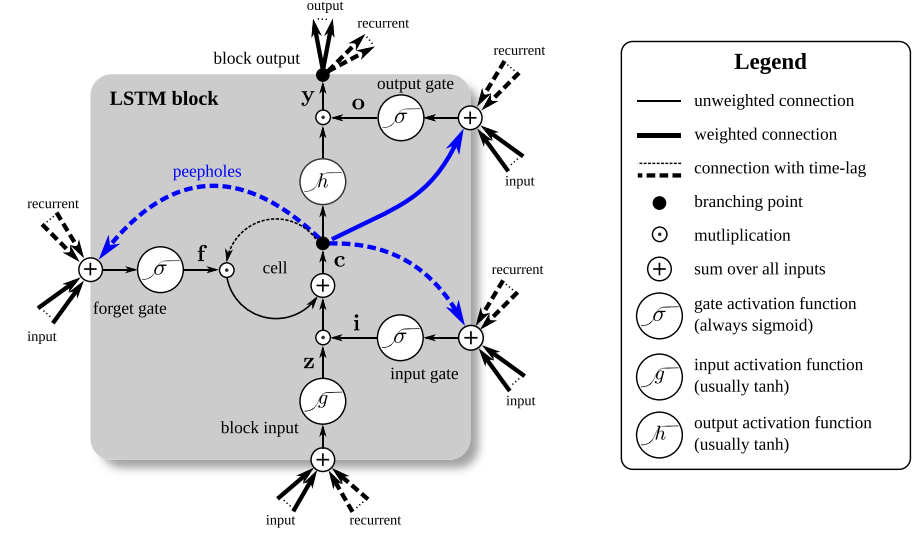
\includegraphics[width=0.9\textwidth]{lstm_cell.png}}
    \end{figure}
\end{frame}

\begin{frame}
\frametitle{LSTM Cell Computation}
\begin{itemize}
	\item The formulas for a vanilla LSTM layer forward pass can be written as:
	\begin{align*}
		&\bar{z}^t = W_z x^t + R_z y^{t-1} + b_z& \\
		&z^t = g(\bar{z}^t)& \text{block input} \\
		&\bar{i}^t = W_i x^t + R_i y^{t-1} + p_i \odot c^{t-1} + b_i& \\
		&i^t = \sigma (\bar{i}^t)& \text{input gate} \\
		&\bar{f}^t = W_f x^t + R_f y^{t-1} + p_f \odot c^{t-1} + b_f& \\
		&f^t = \sigma (\bar{f}^t)& \text{forget gate} \\
		&c^t = z^t \odot i^t + c^{t-1} \odot f^t& \text{cell} \\
		&\bar{o}^t = W_o x^t + R_o y^{t-1} + p_o \odot c^{t-1} + b_o& \\
		&o^t = \sigma (\bar{o}^t)& \text{output gate} \\
		&y^t = h(c^t) \odot o^t& \text{block output}
	\end{align*}
\end{itemize}
\end{frame}

\begin{frame}
\frametitle{LSTM Gates}
\begin{itemize}
	\item Each gate is computed in terms of the current input, the previous output, a peephole connection to the previous cell state and a bias
	\item \(i^t\), \(f^t\) and \(o^t\) are called the input, forget and output gates and their role is to determine how much information flows from previous and current timesteps. This effect is achieved by squashing the gates through a sigmoid function. Then an element wise multiplication is performed such that the input gate determines how much of the current information is used, the forget gate deals with the information flow from the previous cell state and finally, the output gate specifies how much information to send to the output \(y\)
	\item The peephole connections were added such that the network can learn precise timings easier
\end{itemize}
\end{frame}

\end{document}